\documentclass[ignorenonframetext,]{beamer}
\setbeamertemplate{caption}[numbered]
\setbeamertemplate{caption label separator}{: }
\setbeamercolor{caption name}{fg=normal text.fg}
\beamertemplatenavigationsymbolsempty
\usepackage{lmodern}
\usepackage{amssymb,amsmath}
\usepackage{ifxetex,ifluatex}
\usepackage{fixltx2e} % provides \textsubscript
\ifnum 0\ifxetex 1\fi\ifluatex 1\fi=0 % if pdftex
\usepackage[T1]{fontenc}
\usepackage[utf8]{inputenc}
\else % if luatex or xelatex
\ifxetex
\usepackage{mathspec}
\else
\usepackage{fontspec}
\fi
\defaultfontfeatures{Ligatures=TeX,Scale=MatchLowercase}
\fi
% use upquote if available, for straight quotes in verbatim environments
\IfFileExists{upquote.sty}{\usepackage{upquote}}{}
% use microtype if available
\IfFileExists{microtype.sty}{%
\usepackage{microtype}
\UseMicrotypeSet[protrusion]{basicmath} % disable protrusion for tt fonts
}{}
\newif\ifbibliography
\usepackage{graphicx,grffile}
\makeatletter
\def\maxwidth{\ifdim\Gin@nat@width>\linewidth\linewidth\else\Gin@nat@width\fi}
\def\maxheight{\ifdim\Gin@nat@height>\textheight0.8\textheight\else\Gin@nat@height\fi}
\makeatother
% Scale images if necessary, so that they will not overflow the page
% margins by default, and it is still possible to overwrite the defaults
% using explicit options in \includegraphics[width, height, ...]{}
\setkeys{Gin}{width=\maxwidth,height=\maxheight,keepaspectratio}

% Prevent slide breaks in the middle of a paragraph:
\widowpenalties 1 10000
\raggedbottom

\AtBeginPart{
\let\insertpartnumber\relax
\let\partname\relax
\frame{\partpage}
}
\AtBeginSection{
\ifbibliography
\else
\let\insertsectionnumber\relax
\let\sectionname\relax
\frame{\sectionpage}
\fi
}
\AtBeginSubsection{
\let\insertsubsectionnumber\relax
\let\subsectionname\relax
\frame{\subsectionpage}
}

\setlength{\parindent}{0pt}
\setlength{\parskip}{6pt plus 2pt minus 1pt}
\setlength{\emergencystretch}{3em}  % prevent overfull lines
\providecommand{\tightlist}{%
\setlength{\itemsep}{0pt}\setlength{\parskip}{0pt}}
\setcounter{secnumdepth}{0}
\usepackage{tikz}
\usetikzlibrary{bayesnet}
\usetikzlibrary{arrows}
\usetikzlibrary{cd}
\usepackage{pgfplots}
\usepackage{lastpage}
\usepackage{mathrsfs}
\usepackage[makeroom]{cancel}
\usepackage{wrapfig}
\usetikzlibrary{fit,positioning}
\tikzset{font={\fontsize{9pt}{12}\selectfont}}
\setbeamertemplate{footline}{\begin{flushright}\thepage/\pageref{LastPage}~~.\\\end{flushright}}
\usepackage{bm}
\usepackage{amsmath}
\usepackage{xcolor}
\definecolor{blue1}{HTML}{4466FF}
\definecolor{blue2}{HTML}{0022AA}


\newcommand{\red}[1]{\textcolor{red}{#1}}
\newcommand{\look}[1]{\textcolor{purple}{#1}}
\newcommand{\blue}[1]{\textcolor{blue}{#1}}

\title{Dissertation Defense: Numerical Methods for Approximating
High-Dimensional Posterior Distributions}
\author{Jameson Quinn}
\date{}

\begin{document}
\frame{\titlepage}

\begin{frame}{Big picture overview}

\[P(\theta|x)=\frac{P(x|\theta)P(\theta)}{\int_{\theta'\in\Theta} P(x|\theta')P(\theta')d\theta'}\]
If \(\Theta\) is high-D, any estimator of the denominator that amounts
to numerical integration will fail; variance exponential in dim.

\begin{itemize}
\tightlist
\item
  Chapter 1: online data assimilation on spatiotemporal system
\item
  Chapter 2: new method applicable to latent variable models
\item
  Chapter 3: application of method, extension of existing models
\end{itemize}

\end{frame}

\begin{frame}{Variational Inference}

Approximate posterior with a guide distribution
\(q_{\bm{\phi}}(\bm{\theta})\) and choose \(\bm{\phi}\) to mimize KL:
\[\hat{{\bm{\phi}}}=\mathrm{argmin}_{\bm{\phi}}\left[D_{\mathrm{KL}} \left(\;q_{\bm{\phi}}(\bm{\theta})\;\big|\big|\; p(\bm{\theta}|\bm{x})\;\right)\right].\]
Equivalent to maximizing ELBO:
\[\mathrm{ELBO}({\bm{\phi}}):=E_{q_{\bm{\phi}}}
\left[\mathrm{log} p(\bm{x},\bm{\theta})-\mathrm{log} q_{\bm{\phi}}(\bm{\theta})\right]\]

\end{frame}

\begin{frame}{Pyro}

Released in 2017 and still under very active development, pyro is a
cutting-edge python package for black-box VI. * Automatic
differentiation via PyTorch ML * Stochastic optimization * BBVI seems
empirically robust

\end{frame}

\begin{frame}{Problem with existing (mainstream) VI method}

This talk will focus on MVN guide families.

A common assumption is posterior independence of parameters, referred to
as ``meanfield'' guides. Problem:

\begin{center}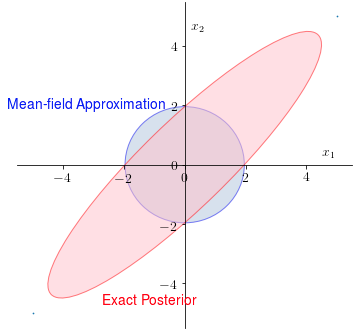
\includegraphics[width=150px]{meanfield_covar_figure} \end{center}

\end{frame}

\begin{frame}{Introduce Laplace family VI (1)}

Among MVN guide families: * Set of all normals, unrestricted covariance,
is too big * Meanfield subset doesn't actually contain any good
approximations * We want subfamily that contains at least some good
approximations without being too big

\end{frame}

\begin{frame}{Introduce Laplace family VI (2)}

Let's guarantee that the family contains the Laplace approximation
around any posterior mode.

Define covariance matrix using observed information of posterior;
negative of Hessian of unnormalized log-density:

\(\mathcal{I}_p\left(\bm{\theta}^*\right) := -H\left[\log p(\bm{\theta})\right]\bigg\rvert_{\bm{\theta}^*}\)

\end{frame}

\begin{frame}{Boosting}

\(\mathcal{I}_p\) not guaranteed to be positive definite. So define
``boosting'' function \(f(\mathcal{I}_p)\) s.t.: * Smooth almost
everywhere. * \(f(\mathcal{I}_p)\approx\mathcal{I}_p\) if
\(\mathcal{I}_p\) already p.d. A similar problem arises in optimization
(quasi-Newton methods); solved via modified Cholesky algorithms (Fang,
2008)

Furthermore, we can parametrize \(f\) to create a boosting family
\(f_{\bm{\psi}}\), for \(\psi_i>0\), s.t.: * Each dimension of
\(\bm{\psi}\) corresponds to a model parameter * As
\(\bm{\psi}\rightarrow\vec{\bm{0}}\) from above,
\(f(\mathcal{I}_p)\rightarrow\mathcal{I}_p\) if \(\mathcal{I}_p\)
already p.d.

\end{frame}

\begin{frame}{Formal definition of Laplace family (1)}

Let \(p(\bm{\theta})\) be a (possibly unnormalized) probability
distribution on \(\mathbb{R}^d\). Let \(\Theta \subseteq \mathbb{R}^d\),
\(\Psi \subseteq \mathbb{R}^D_+\), and let \(f_\Psi\) be a boosting
family.

The Laplace guide family \(\mathcal{L}_{\Theta\times\Psi} (p,f_\Psi)\)
is the set of \(d\)-dimesnional normal distributions
\(\{q_{\bm{\theta}^*,\bm{\psi}}:\bm{\theta}^*\in\Theta,\;\bm{\psi}\in\Psi\}\),
where \(q_{\bm{\theta}^*,\bm{\psi}}\) has mean \(\bm{\theta}^*\) and
precision matrix \(f_{\bm{\psi}} \left(\I_p(\bm{\theta}^*)\right)\).\}

\end{frame}

\begin{frame}{Toy model results}

Nice picture of toy model

\end{frame}

\begin{frame}{Latent variable models (or: why hi-D?)}

Define, including defining Gamma and Theta This is why we need a
high-dimensional solution.

\end{frame}

\begin{frame}{Block arrowhead matrices}

Show block-arrowhead matrix, say it's easy to sample from and easy to
boost (don't write anything down for this, just point)

\end{frame}

\begin{frame}{Additional methods for LV models: subsampling}

Explain subsampling Mention weights, say we haven't yet implemented them
anywhere think about exactly what you want to say about its
qusi-unbiasedness (have hidden slides with slide with details) Explain
amortization: restricting to subspace of the guide where latents are
approximate MLEs relative to globals, guide parameters are now just
gamma, psi\_gamma, psi\_lambda (possibly mention Newton's method, but
Mira thinks not) (Say that they go together nicely, but don't go into
detail)

\end{frame}

\begin{frame}{Additional methods for LV models: boosting}

\end{frame}

\begin{frame}{Ch 1 Results}

Improved version from thesis Very brief explanation only, but mention
transforming parameters

\end{frame}

\begin{frame}{Ch 2: Ecological inference. Introduction}

Mainly comes up in voting rights cases, so I'll talk about it in this
setting Explain problem in the abstract by showing pictures of matrices
and talking about them (you don't need much else on this slide)

\end{frame}

\begin{frame}{EI: example matrices}

\end{frame}

\begin{frame}{Relevance: Thornburg v. Gingles}

Mention Gingles SCOTUS case briefly show Gingles graph

\end{frame}

\begin{frame}{History of attempted solutions: ER}

Picture of Brexit ER Explain problem with this method

\end{frame}

\begin{frame}{King's EI: 2x2 case (1)}

Describe Point out innovation of looking at latents rather than globals

\end{frame}

\begin{frame}{King's EI: 2x2 case (2)}

\end{frame}

\begin{frame}{Rosen, Jiang, King, \& Tanner: RxC case (1)}

Explain model

\end{frame}

\begin{frame}{Rosen, Jiang, King, \& Tanner: RxC case (1)}

\end{frame}

\begin{frame}{Limitations of RJKT\ldots{}}

it's cheating (applies racial constraints at wrong level of hierarchy,
because they don't know how to apply both vote-total and racial
constraints at same level; I'll solve this with polytopize) hard to
extend model (give examples of how you might extend it) relies on MCMC,
so if you extend by a lot will be too slow

\end{frame}

\begin{frame}{\ldots{}and our contribution}

No cheating (polytope) More flexible model VI instead of MCMC (make this
slide parallel to previous one)

\end{frame}

\begin{frame}{Our model}

Talk briefly about how you could add other Christmas tree ornaments Talk
about why this is hard to make a guide for

\end{frame}

\begin{frame}{Modified model}

Cmult Polytopize: ae smooth map from R\^{}n to polytope Pseudovoters
because of boundary issues that arise from Cmult and polytopize; don't
go into details

All of these make the model itself slightly less-realistic, but make VI
work.

\end{frame}

\begin{frame}{Polytopize (1)}

two nice pictures from thesis formula written down

\end{frame}

\begin{frame}{Polytopize (2)}

\end{frame}

\begin{frame}{Guide, with amortization}

picture from paper, but remade to look more sane!!!! Maybe a list of
things to note (changes form model)

\end{frame}

\begin{frame}{Testing our EI on simulated data}

Describe how we got the simulated NC data actual demographics realistic
alpha and beta we get to experiment sigma\_nu

\end{frame}

\begin{frame}{EI results (1)}

Show updated tables from paper Point out that this is different
(better!) than what you originally sent, because: does not underestimate
variance (fixed bug) corrected alphas and betas (so that overall
percentages of people of each race voting for each candidate approximate
the true 2016 data, as intended) improved amortization (optimize Y →
optimize W)

Conclusion: We are as good as RJKT, but we're just getting started

\end{frame}

\begin{frame}{EI results (2)}

\end{frame}

\begin{frame}{Discussion/future work (Ch. 3)}

Including the covariate Multiple elections Actual NC data Compare
hierachical model without EI, Standard RJKT, and our model
Cross-validation Say that this is the stuff we plan to include in final
paper

\end{frame}

\begin{frame}{Discussion/future work (Ch. 2)}

More on subsampling: general theory of how to assign weights to minimize
variance of estimator in subsampling (use Ch 3 as example) maybe some
theory to help choose sample size for SVI Replace normal with T in guide
Say that this will not be in current paper, which is basically done

\end{frame}

\begin{frame}{Thanks}

\end{frame}

\begin{frame}{Directory of extra slides}

\end{frame}

\begin{frame}{Non-meanfield prior work}

Just the list from the paper Give example of actual theorem you can
prove when you have conjugate model structure

\end{frame}

\begin{frame}{Details on toy model}

Just the model

\end{frame}

\begin{frame}{More on block-arrowhead matrices}

Formulas for boosting Formulas for sampling

(basically just the stuff in the appendix)

\end{frame}

\begin{frame}{What we expect from subsampling}

HARD

\end{frame}

\begin{frame}{Details of ECHS}

The actual model Result tables

\end{frame}

\begin{frame}{More details on RJKT}

\end{frame}

\begin{frame}{Possible extensions to our EI model}

\end{frame}

\begin{frame}{Boundary issues with polytope; pseudovoters}

HARD

\end{frame}

\begin{frame}{How our EI amortization works (1)}

Which variables are we amortizing: Y, nu, sigma\_nu Steps: Find
approximate mode of p(Y\textbar{}alpha, beta, nu) constrained to lie on
polytope (this is linear algebra plus stirling's approximation)
One-dimensional Newton's method to find approximate mode of W. (Not the
same thing, because there's Jacobian, mode of W is further away from
boundary) Find approximate mode of p(nu, sigma\_nu\textbar{} gamma, W)
Newton's method (for free!!)

\end{frame}

\begin{frame}{How our EI amortization works (2)}

Details on how we get nu and sigma\_nu

\end{frame}

\begin{frame}{More EI results}

\end{frame}

\begin{frame}{END DEFENSE, START OLD PRESENTATION}

\end{frame}

\begin{frame}{Teaser}

\includegraphics{defense_files/figure-beamer/unnamed-chunk-7-1.pdf}

\end{frame}

\begin{frame}{Thornburg v Gingles, 1986}

A majority-minority district must be created if:

\begin{enumerate}
\def\labelenumi{\arabic{enumi}.}
\item
  A minority group is ``sufficiently numerous and compact to form a
  majority in a single-member district''; and
\item
  The minority group is \red{\textbf{"politically cohesive"}}; and
\item
  The ``majority \red{\textbf{votes sufficiently as a bloc}} to enable
  it \ldots{} usually to defeat the minority's preferred candidate.''
\end{enumerate}

\end{frame}

\begin{frame}{Ecological data}

\begin{tikzpicture}[
squared notebook/.pic={\clip[postaction={shade,left color=white}](0,0) rectangle (6.5,4);
\draw[ultra thick](0,0) rectangle (6.5,4);}
]
\foreach \x in {2,1.75,1.5,1.25,1,.75,0.5,.25,0}\pic at (\x,\x){squared notebook};
\draw[-latex] (7,0) -- +(1.5,1.5) node[below right,midway,rotate=45] {precinct};
\node[rotate=90] (h) at (.5,2) {Race};
\node (w) at (3.5,3.5) {Candidate};



\node (w) at (3.5,2) {$\begin{array}{l|lll|l}
& R & D & No & \\
\hline
White & \red{?} & \red{?} & \red{?} & 400 \\
Black & \red{?} & \red{?} & \red{?} & 200   \\
Hispanic & \red{?} & \red{?} & \red{?} & 100   \\
Other & \red{?} & \red{?} & \red{?} & 100   \\
\hline
 & 400 & 200 & 200 & 800\end{array}$};

\end{tikzpicture}

\end{frame}

\begin{frame}{Majority=Majority?}

\begin{tikzpicture}[
squared notebook/.pic={\clip[postaction={shade,left color=white}](0,0) rectangle (6.5,4);
\draw[ultra thick](0,0) rectangle (6.5,4);}
]
\foreach \x in {2,1.75,1.5,1.25,1,.75,0.5,.25,0}\pic at (\x,\x){squared notebook};
\draw[-latex] (7,0) -- +(1.5,1.5) node[below right,midway,rotate=45] {precinct};
\node[rotate=90] (h) at (.5,2) {Race};
\node (w) at (3.5,3.5) {Candidate};



\node (w) at (3.5,2) {$\begin{array}{l|lll|l}
& R & D & No & \\
\hline
White & \red{400} & 0 & 0 & 400 \\
Black & 0 & \red{200} & 0 & 200   \\
Hispanic & 0 & 0 & \red{100} & 100   \\
Other & 0 & 0 & \red{100} & 100   \\
\hline
 & 400 & 200 & 200 & 800\end{array}$};

\end{tikzpicture}

\end{frame}

\begin{frame}{Backwards?}

\begin{tikzpicture}[
squared notebook/.pic={\clip[postaction={shade,left color=white}](0,0) rectangle (6.5,4);
\draw[ultra thick](0,0) rectangle (6.5,4);}
]
\foreach \x in {2,1.75,1.5,1.25,1,.75,0.5,.25,0}\pic at (\x,\x){squared notebook};
\draw[-latex] (7,0) -- +(1.5,1.5) node[below right,midway,rotate=45] {precinct};
\node[rotate=90] (h) at (.5,2) {Race};
\node (w) at (3.5,3.5) {Candidate};



\node (w) at (3.5,2) {$\begin{array}{l|lll|l}
& R & D & No & \\
\hline
White & 0 & \red{200} & \red{200} & 400 \\
Black & \red{200} & 0 & 0 & 200   \\
Hispanic & \red{100} & 0 & 0 & 100   \\
Other & \red{100} & 0 & 0 & 100   \\
\hline
 & 400 & 200 & 200 & 800\end{array}$};

\end{tikzpicture}

\end{frame}

\begin{frame}{Independence?}

\begin{tikzpicture}[
squared notebook/.pic={\clip[postaction={shade,left color=white}](0,0) rectangle (6.5,4);
\draw[ultra thick](0,0) rectangle (6.5,4);}
]
\foreach \x in {2,1.75,1.5,1.25,1,.75,0.5,.25,0}\pic at (\x,\x){squared notebook};
\draw[-latex] (7,0) -- +(1.5,1.5) node[below right,midway,rotate=45] {\look{precinct}};
\node[rotate=90] (h) at (.5,2) {Race};
\node (w) at (3.5,3.5) {\look{Candidate}};



\node (w) at (3.5,2) {$\begin{array}{l|lll|l}
& R & D & No & \\
\hline
White & \red{200} & \red{100} & \red{100} & 400 \\
Black & \red{100} & \red{50} & \red{50} & 200   \\
Hispanic & \red{50} & \red{25} & \red{25} & 100   \\
Other & \red{50} & \red{25} & \red{25} & 100   \\
\hline
 & 400 & 200 & 200 & 800\end{array}$};

\end{tikzpicture}

\end{frame}

\begin{frame}{Structure}

\begin{itemize}
\tightlist
\item
  Pose the ecological problem (done)
\item
  Quick review of prior approaches
\item
  A basic, extensible model for EI
\item
  Why and how to reparameterize
\item
  Review of variational inference
\item
  Applying variational inference to EI
\item
  Guide (aka variational distribution) based on observed information
\end{itemize}

\end{frame}

\begin{frame}{Ecological regression (for \(2\times 2\) cases)}

\includegraphics{defense_files/figure-beamer/unnamed-chunk-8-1.pdf}

Brexit voting data. (Example from ``The Stats Guy'' blog by Adam
Jacobs.) Valid under certain (strong) assumptions.

\end{frame}

\begin{frame}{Ecological regression: uh oh}

\includegraphics{defense_files/figure-beamer/unnamed-chunk-9-1.pdf}

Brexit supported by 79\% of people without a degree\ldots{} and -16\% of
those with one??? Ecological fallacy, Simpson's paradox, etc.

\end{frame}

\begin{frame}{Infer latents, not parameters}

Insight from King, Rosen, Tanner 1999: instead of focusing on population
parameters, which are not directly constrained by the data, focus on
latent parameters, which are.

Refined by Rosen, King, Jiang, Tanner (2001):

\begin{itemize}
\item
  Fully Bayesian model
\item
  extends to \(R\neq 2 \neq C\)
\item
  fast, moment-based estimator
\item
  now widely used.
\end{itemize}

\end{frame}

\begin{frame}{Issues with RKJT 2001:}

The RKJT model can, in principle, be extended to handle additional
factors such as:

\begin{itemize}
\tightlist
\item
  inter-row or inter-column correlations
\item
  covariates
\item
  multiple elections
\item
  exit polling data
\item
  etc.
\end{itemize}

However:

\begin{itemize}
\tightlist
\item
  the moment-based estimator breaks down,
\item
  MCMC on such a high-dimensional latent space can be challenging.
\end{itemize}

\end{frame}

\begin{frame}{Flexible model (1)}

\begin{tikzpicture}
  % Define nodes
  \node[latent]           (beta) {$\bm{\beta}_r$};
  \node[const, above=0.4 of beta] (rbighide) {};
  \node[latent, above=of beta] (sdb) {$\sigma_\beta$};
  \node[latent, left=of beta]  (alpha) {$\bm{\alpha}$};
  \node[latent, right=2 of beta]            (gamma) {$\bm{\gamma}_{u,r}$};
  \node[latent, above=of gamma] (sdg) {$\sigma_\gamma$};
  \node[det, below=.7of gamma]            (pi) {$\bm{\pi}_{u,r}$};
  \factor[below=.4 of pi] {multi} {right:$\mathrm{Multi}$} {} {};
  \node[obs, left=of multi]            (n) {$n_{u,r}$};
  \node[latent, below=.5 of multi]            (y) {$\bm{y}_{u,r}$};
  \node[obs, diamond, below=of y]            (v) {$\bm{v}_{u}$};
  \node[const, right=0.6 of y] (ubighide) {};
  \node[const, right=1.2 of y] (rbighide) {};

  % Connect the nodes
  \edge {sdb} {beta} ;
  \edge {sdg} {gamma} ; 
  \edge {alpha,beta,gamma} {pi} ;
  \factoredge {pi,n} {multi} {y} ; 
  \edge {y} {v} ;

  % Plates
  \plate {U} {(gamma)(y)(multi)(pi)(n)(v)(ubighide)} {$U$} ;
  \plate {R} {(beta)(gamma)(y)(rbighide)(U.north east)} {$R$} ;
\end{tikzpicture}

\end{frame}

\begin{frame}{Flexible model (2)}

\begin{tikzpicture}
  % Define nodes
  \node[latent]           (beta) {$\bm{\beta}_r$};
  \node[const, above=0.4 of beta] (rbighide) {};
  \node[latent, above=of beta] (sdb) {$\sigma_\beta$};
  \node[latent, left=of beta]  (alpha) {$\bm{\alpha}$};
  \node[latent, right=2 of beta]            (gamma) {$\bm{\gamma}_{u,r}$};
  \node[latent, above=of gamma] (sdg) {$\sigma_\gamma$};
  \node[det, below=.7of gamma]            (pi) {$\bm{\pi}_{u,r}$};
  \factor[below=.4 of pi] {multi} {right:$\color{red}{\mathrm{CMult}}$} {} {};
  \node[obs, left=of multi]            (n) {$n_{u,r}$};
  \node[latent, below=.5 of multi]            (y) {$\bm{y}_{u,r}$};
  \node[const, right=0.8 of y] (ubighide) {};
  \node[const, right=1.4 of y] (rbighide) {};
  \node[det, below=of y]            (W) {$\color{red}{W_{u}}$};
  \node[obs, diamond, left=.66 of W]            (v) {$\bm{v}_{u}$};

  % Connect the nodes
  \edge {sdb} {beta} ;
  \edge {sdg} {gamma}; 
  \edge {alpha,beta,gamma} {pi} ;
  \factoredge {pi,n} {multi} {y} ; 
  \edge[] {y} {W} ; 
  \edge[] {v} {W} ; 
  \edge[] {y} {v} ; 

  % Plates
  \plate {U} {(gamma)(y)(multi)(pi)(n)(W)(v)(ubighide)} {$U$} ;
  \plate {R} {(beta)(gamma)(y)(rbighide)(U.north east)} {$R$} ;
\end{tikzpicture}

\end{frame}

\begin{frame}{Flexible model (3)}

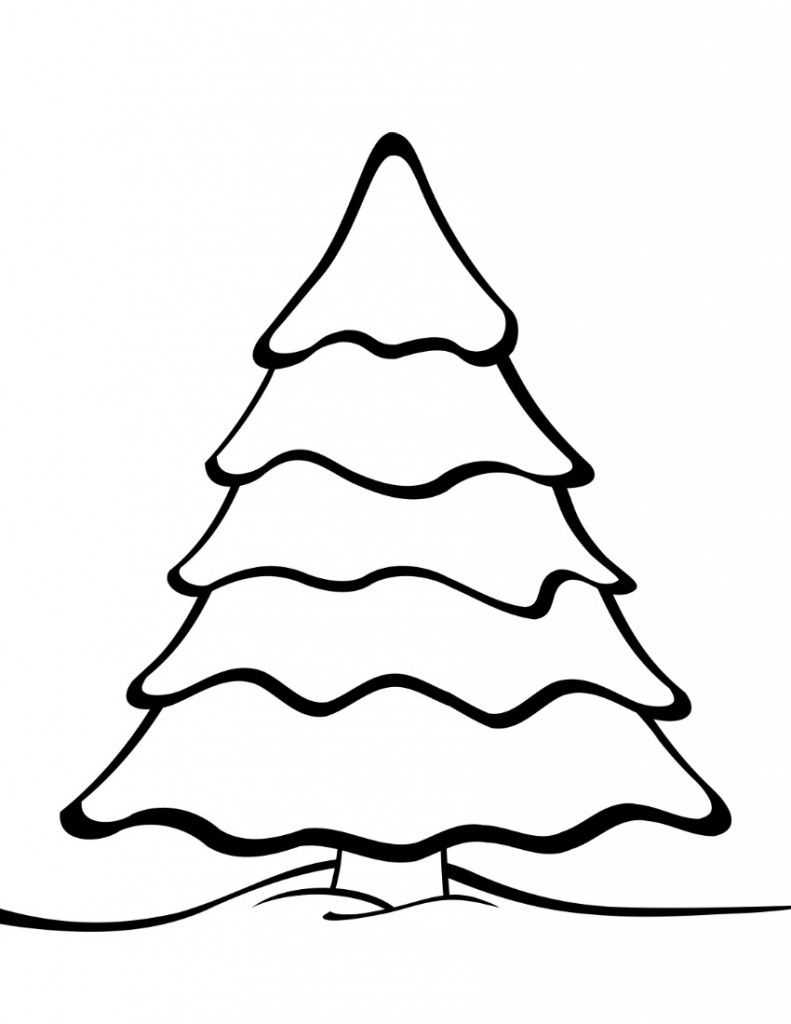
\includegraphics[width=0.30000\textwidth]{holidaytree_bare.jpg}

\includegraphics[width=0.30000\textwidth]{holidaytree_decorated.png}

\[\vec{y}_{p,r}=y_{p,r,c}\Vert_{c=1}^C\sim \operatorname{CMult}\left(n_{p,r},\frac{exp(\alpha_c+\beta_{r,c}\red{+\lambda_{r,c,p}})\Vert_{c=1}^C}{\sum_{c=1}^Cexp(\alpha_c+\beta_{r,c}\red{+\lambda_{r,c,p}})}\right)\]

\[\alpha_c\sim\mathcal{N}(0,\sigma_\alpha)~~~~~~~\sigma_\alpha\sim\operatorname{Expo}(5)\]

\[\beta_{r,c}\sim\mathcal{N}(0,\sigma_\beta)~~~~~~~\sigma_\beta\sim\operatorname{Expo}(5)\]

\[\red{\lambda_{r,c,p}\sim\mathcal{N}(0,\sigma_\beta)}~~~~~~~\sigma_\lambda\sim\operatorname{Expo}(5)\]
\(\lambda\) handles overdispersion. Note: Bayesian Occam's Razor.

\end{frame}

\begin{frame}{Standard Bayesian approach (simplified)}

\(\begin{array}{cl} \operatorname{priors}~\pi & \\ \downarrow & \\ \operatorname{parameters}~\theta & \\ \downarrow & \\ \operatorname{latent~variables}~y & \\ \downarrow & \\ \operatorname{data}~z & \end{array}\)

\end{frame}

\begin{frame}{Standard Bayesian approach (cont'd)}

\(\begin{array}{cl} \operatorname{priors}~\pi & \\ \downarrow & \operatorname{(parameterizes~distribution)}\\ \operatorname{parameters}~\theta & \operatorname{(unobservable~quantities~of~interest;~low-D)}\\ \downarrow & \operatorname{(parameterizes~distribution)}\\ \operatorname{latent~variables}~y & \operatorname{(unobservable~nuisance~parameters;~high-D)}\\ \downarrow & \operatorname{(parameterizes~distribution)}\\ \operatorname{data}~z & \end{array}\)

\end{frame}

\begin{frame}{Ecological Inference}

\(\begin{array}{cl} \operatorname{priors}~\pi & \\ \downarrow & \operatorname{(parameterizes~distribution)}\\ \operatorname{parameters}~\theta & \operatorname{(unobservable~\red{nuisance~parameters};~low-D\red{?})}\\ \downarrow & \operatorname{(parameterizes~distribution)}\\ \operatorname{latent~variables}~y & \operatorname{(unobserv\red{ed~quantities~of~interest};~high-D)}\\ \downarrow & \operatorname{\red{(deterministic~function)}}\\ \operatorname{data}~z & \end{array}\)

A likelihood from a deterministic function is an indicator function!

\end{frame}

\begin{frame}{Ecological case}

Since the likelihood is just an indicator function, the posterior is
just the prior, restricted to the set of values where the likelihood is
1 and renormalized. For each precinct, this set turns out to be a
polytope \(\mathcal{Y}_{z_p}\) in an \((R-1)(C-1)\) dimensional subspace
of the full \(\mathbb{R}^{RC}\).

\begin{tikzpicture}[
squared notebook/.pic={\clip[postaction={shade,left color=white}](0,0) rectangle (4,4);
\draw[ultra thick](0,0) rectangle (4,4);}
]
\foreach \x in {.75,0.5,.25,0}\pic at (\x,\x){squared notebook};
\node[rotate=90] (h) at (.2,2) {Race};
\node (w) at (2,3.5) {Candidate};



\node (w) at (2.2,2) {$\begin{array}{lll|l}
R & D & No & \\
\hline
\textcolor{red}{y_{p11}} & \textcolor{blue}{y_{p12}} & y_{p13} & \textcolor{olive}{500} \\
y_{p21} & y_{p22} & y_{p23} & \textcolor{purple}{700}   \\
\hline
\textcolor{red}{400} & \textcolor{blue}{400} & 400 & 1200\end{array}$};











\node[] at (8, -1.1)   (c) {$\mathcal{Y}_{z_p}\subset\mathbb{R}^{(R-1)(C-1)}\longleftrightarrow\mathbb{R}^{RC} $};

%polytope
\draw[style=-] (7,0) -- +(-1,1) node[below left=.25cm,anchor=base,midway,rotate=-45] {$y_{p11}+y_{p12}>\textcolor{purple}{100}$};
\draw[style=-] (7,0) -- +(3,0) node[below=.3cm,anchor=base,midway] {$\textcolor{blue}{y_{p12}}>0$};
\draw[style=-] (10,0) -- +(0,1) node[right = .3cm,anchor=base,midway,rotate=90] {$\textcolor{red}{y_{p11}<400}$};
\draw[style=-] (10,1) -- +(-3,3) node[above right=.15cm,anchor=base,midway,rotate=-45] {$y_{p11}+y_{p12}<\textcolor{olive}{500}$};
\draw[style=-] (7,4) -- +(-1,0) node[above=.2cm,anchor=base,midway] {$\textcolor{blue}{y_{p12}<400}$};
\draw[style=-] (6,1) -- +(0,3) node[left = .2cm,anchor=base,midway,rotate=90] {$\textcolor{red}{y_{p11}}>0$};


\end{tikzpicture}

\end{frame}

\begin{frame}{Independence point}

\begin{tikzpicture}[
squared notebook/.pic={\clip[postaction={shade,left color=white}](0,0) rectangle (4,4);
\draw[ultra thick](0,0) rectangle (4,4);}
]
\foreach \x in {.75,0.5,.25,0}\pic at (\x,\x){squared notebook};
\node[rotate=90] (h) at (.2,2) {Race};
\node (w) at (2,3.5) {Candidate};



\node (w) at (2.2,2) {$\begin{array}{lll|l}
R & D & No & \\
\hline
\red{167} & \red{167} & 167 & 500 \\
233 & 233 & 233 & 700   \\
\hline
400 & 400 & 400 & 1200\end{array}$};



\draw[red,fill=red] (7.667,1.667) circle (.5ex);

\node[] at (7.667,1.267)   (c) {Independence};

%\tkzDefPoint(7.667,1.667){M}
%\tkzLabelPoint[right,below](M){Independence}






\node[] at (8, -1.1)   (c) {$\mathcal{Y}_{z_p}\subset\mathbb{R}^{(R-1)(C-1)}\longleftrightarrow\mathbb{R}^{RC}$};

%polytope
\draw[style=-] (7,0) -- +(-1,1) node[below left=.25cm,anchor=base,midway,rotate=-45] {$y_{p11}+y_{p12}>\textcolor{black}{100}$};
\draw[style=-] (7,0) -- +(3,0) node[below=.3cm,anchor=base,midway] {$\textcolor{black}{y_{p12}}>0$};
\draw[style=-] (10,0) -- +(0,1) node[right = .3cm,anchor=base,midway,rotate=90] {$\textcolor{black}{y_{p11}<400}$};
\draw[style=-] (10,1) -- +(-3,3) node[above right=.15cm,anchor=base,midway,rotate=-45] {$y_{p11}+y_{p12}<\textcolor{black}{500}$};
\draw[style=-] (7,4) -- +(-1,0) node[above=.2cm,anchor=base,midway] {$\textcolor{black}{y_{p12}<400}$};
\draw[style=-] (6,1) -- +(0,3) node[left = .2cm,anchor=base,midway,rotate=90] {$\textcolor{black}{y_{p11}}>0$};


\end{tikzpicture}

\end{frame}

\begin{frame}{Diffeomorphic function
\(g(y'):\mathbb{R}^{(R-1)(C-1)}\rightarrow\mathcal{Y}_{z_p}\)}

\begin{tikzpicture}

%axes
\draw[-latex] (2,2) -- +(2,0) node[below right,midway,rotate=45] {};
\draw[-latex] (2,2) -- +(-2,0) node[below right,midway,rotate=45] {};
\draw[-latex] (2,2) -- +(0,2) node[below right,midway,rotate=45] {};
\draw[-latex] (2,2) -- +(0,-2) node[below right,midway,rotate=45] {};

%vectors in y'
\draw[-latex] (2,2) -- +(.3,.4) node[below right,midway,rotate=45] {};
\draw[-latex] (2.3,2.4) -- +(.3,.4) node[below right,midway,rotate=45] {};
\draw[-latex] (2.6,2.8) -- +(.3,.4) node[below right,midway,rotate=45] {};
\draw[-latex] (2.9,3.2) -- +(.3,.4) node[below right,midway,rotate=45] {};


\draw[-latex] (2,2) -- +(-.4,-.3) node[below right,midway,rotate=45] {};
\draw[-latex] (1.6,1.7) -- +(-.4,-.3) node[below right,midway,rotate=45] {};
\draw[-latex] (1.2,1.4) -- +(-.4,-.3) node[below right,midway,rotate=45] {};
\draw[-latex] (0.8,1.1) -- +(-.4,-.3) node[below right,midway,rotate=45] {};

\draw[-latex] (2,2) -- +(.5,0) node[below right,midway,rotate=45] {};
\draw[-latex] (2.5,2) -- +(.5,0) node[below right,midway,rotate=45] {};
\draw[-latex] (3,2) -- +(.5,0) node[below right,midway,rotate=45] {};
\draw[-latex] (3.5,2) -- +(.5,0) node[below right,midway,rotate=45] {};

%function connector
\node[] at (5, -.7)   (a) {$g(y')$};
\node[] at (5, -1.1)   (b) {$\longrightarrow$};

%labels for spaces
\node[] at (2, -1.1)   (c) {$\mathbb{R}^{(R-1)(C-1)}$};
\node[] at (8, -1.1)   (c) {$\mathcal{Y}_{z_p}\subset\mathbb{R}^{(R-1)(C-1)}\longleftrightarrow\mathbb{R}^{RC}$};


%polytope
\draw[style=-] (7,0) -- +(-1,1) node[below left=.25cm,anchor=base,midway,rotate=-45] {$y_{p11}+y_{p12}>100$};
\draw[style=-] (7,0) -- +(3,0) node[below=.3cm,anchor=base,midway] {$y_{p12}>0$};
\draw[style=-] (10,0) -- +(0,1) node[right = .3cm,anchor=base,midway,rotate=90] {$y_{p11}<400$};
\draw[style=-] (10,1) -- +(-3,3) node[above right=.15cm,anchor=base,midway,rotate=-45] {$y_{p11}+y_{p12}<500$};
\draw[style=-] (7,4) -- +(-1,0) node[above=.2cm,anchor=base,midway] {$y_{p12}<400$};
\draw[style=-] (6,1) -- +(0,3) node[left = .2cm,anchor=base,midway,rotate=90] {$y_{p11}>0$};


%vectors in polytope
\draw[-latex] (7.5,1.5) -- +(.3,.4) node[below right,midway,rotate=45] {};
\draw[-latex] (7.8,1.9) -- +(.2,.266) node[below right,midway,rotate=45] {};
\draw[-latex] (8.0,2.166) -- +(.133,.177) node[below right,midway,rotate=45] {};
\draw[-latex] (8.133,2.344) -- +(.0889,.1185) node[below right,midway,rotate=45] {};



\draw[-latex] (7.5,1.5) -- +(-.4,-.3) node[below right,midway,rotate=45] {};
\draw[-latex] (7.1,1.2) -- +(-.2667,-.2) node[below right,midway,rotate=45] {};
\draw[-latex] (6.833,1.0) -- +(-.1778,-.133) node[below right,midway,rotate=45] {};
\draw[-latex] (6.655,.866) -- +(-.1185,-.0889) node[below right,midway,rotate=45] {};

\draw[-latex] (7.5,1.5) -- +(.5,0) node[below right,midway,rotate=45] {};
\draw[-latex] (8,1.5) -- +(.375,0) node[below right,midway,rotate=45] {};
\draw[-latex] (8.375,1.5) -- +(.281,0) node[below right,midway,rotate=45] {};
\draw[-latex] (8.656,1.5) -- +(.211,0) node[below right,midway,rotate=45] {};

%dots at 0,0 and independence

\draw[red,fill=red] (7.5,1.5) circle (.5ex);
\draw[red,fill=red] (2,2) circle (.5ex);

\end{tikzpicture}

\[\frac{d \Vert g(y')-g(0)\Vert }{d\Vert y'\Vert}=y_{p11}y_{p12}(400-y_{p11})(400-y_{p12})(500-y_{p11}-y_{p12})\cdots\]

\end{frame}

\begin{frame}{Stochastic variational inference (Hoffman et al., 2013)}

Goal: approximate \blue{unnormalized} posterior density
\(p(\theta,y|z)\propto p(z|\theta,y)p_\pi(\theta,y)\) with sampleable
parametric distribution \(q_\phi(\theta,y)\). (Called a \textbf{guide}
in the pyro SVI package for python)

Maximize negative K-L divergence from guide to \blue{normalized}
posterior \(p(z|\theta,y)p_\pi(\theta,y)/p(z)\):

\[E_{q_\phi}\left(\log\frac{p(z|\look{\theta},y)p_{\look{\pi}}(\theta,y)}
{q_\phi(\theta,y)p(z)}\right)<0\]

\[E_{q_\phi}\left(\log[p(z|y)p(\theta,y)]-\log
[q_\phi(\theta,y)]-\look{\log(p(z))}\right)<0\]

\[E_{q_\phi}\left(\log[p(z|y)p(\theta,y)]-\log
[q_\phi(\theta,y)]\right)<\log(p(z))\]

LHS is the \textbf{ELBO}; goal is to find \(\phi\) which maximizes it.

\end{frame}

\begin{frame}{ELBO terms}

\(E_{q_\phi}\left(\log[p(z|y)p(\theta,y)]\right)\) is \textbf{energy}
term. Maximized if \(q\) is a \(\delta\) (dirac mass) at MLE for
\((\theta,y|z)\). Unboundedly negative if \(q\) has probability mass
where \(p\) doesn't.

\(E_{q_\phi}\left(-\log[q_\phi(\theta,y)]\right)\) is \textbf{entropy}
term. Maximized by making q diffuse. For example, if \(q\) is
\(\mathcal{N}(\bm{\mu},\Sigma)\), then this is inversely proportional to
\(\mathrm{det}(\Sigma)\). In principle unboundedly negative, but in
practice, it's easier to control than energy term.

Together, they're maximized if \(q_\phi\) ``imitates'' \(p\).

\includegraphics{defense_files/figure-beamer/unnamed-chunk-10-1.pdf}

\end{frame}

\begin{frame}{EI case}

Reparameterize with \(y=g(y')\), and approximate \(p(\theta,g(y'))]\)
using \(q_{\phi,z}(\theta,y')\). ELBO over \(y'\) then becomes:

\[E_{q_{\phi,z}}\left(\log[p(\theta,g(y'))\operatorname{det}(J(g(y')))]-\vphantom{\Big|}\log
[q_{\phi,z}(\theta,y')]\right)\]

A common form of variational inference uses a ``mean field'' guide which
factorizes across all parameters and latents; frequently, one that's
Normal in each dimension. This ignores the dependence induced by
conditioning on the data; which is particularly strong in the case of
EI.

\end{frame}

\begin{frame}{Laplace family}


\includegraphics[width=60px]{stay_puft_2} \emph{``Choose the form of
your posterior''}

Take \(q(\theta,y')\) to be a multivariate Normal, and assume that once
the ELBO is maximized, its mode \((\hat{\theta},\hat{y})\) coincides
with a mode of the posterior. What should its covariance matrix be?

There's an obvious way to approximate a twice-differentiable,
unnormalized distribution with a Normal: a Laplace approximation.

That is, use the observed information matrix:

\[\mathscr{I}(\hat{\bm{y}}',\hat{\theta})=D^2\left(\log[p(\hat{\theta},g(\hat{y}'))\operatorname{det}(J(g(y')))]\right)\]
as the precision matrix of \(q\).

\end{frame}

\begin{frame}{Graphical posterior}

\begin{tikzpicture}

  % Define nodes
  \node[const]           (hats) {$\hat{\bm{\theta}}$};
  \node[const, right=2.5 of hats]            (What) {$\hat{W}_{u}$};
  
  \factor[below=of hats,yshift=-.3cm] {paramdist} {right:$\mathcal{N}$} {} {};
  \node[latent, diamond, aspect=2.5, left=.8 of paramdist]            (Iparams) {$\mathscr{I}^{-1}(\hat{\bm{\theta}})$};
  \node[latent, below=of paramdist]            (params) {$\bm{\theta}$};
  
  
  
  \node[const, below=1.5 of What,xshift=-3cm] (stuff) {};
  
  \factor[below=2.11 of What] {fulldist} {above left:$\mathcal{N}$} {} {};
  \node[latent, diamond, aspect=2.5, right=.8 of fulldist]            (Ifull) {$\mathscr{I}^{-1}(\hat{\bm{\theta}},\hat{W}_{u})$};
  \node[latent, below=of fulldist]            (W) {$W_u$};
  \node[const, right=0.3 of W]            (detour) {};
  \node[det, below=0.6 of W]            (gamma) {$\bm{\gamma}_{u,r}$};
  \node[const, below=0.2 of gamma,xshift=-0.8cm]            (uhide) {};

  % Connect the nodes
  \edge[] {hats} {Iparams} ;
  \edge[-] {hats} {paramdist} ; 
  \edge[-] {Iparams} {paramdist} ; 
  \edge {paramdist} {params} ; 
  \edge {hats,What} {Ifull} ;
  \edge[-] {params} {fulldist}; 
  \edge[-] {Ifull} {fulldist}  ; 
  \edge[-] {What} {fulldist} ; 
  \edge {fulldist} {W} ; 
  \edge[] {W,params} {gamma} ;

  % Plates
  \plate {U} {(gamma)} {$R$} ;
  \plate {U} {(Ifull)(fulldist)(W)(gamma)(uhide)(What)} {$U$} ;
\end{tikzpicture}

\end{frame}

\begin{frame}{Computability}

\begin{itemize}
\tightlist
\item
  Using pyro, a variational inference package for python.
\item
  \(\mathscr{I}(\hat{\bm{y}}',\hat{\theta})\) can be calculated using
  automated differentiation.
\item
  \(\mathscr{I}(\hat{\bm{y}}',\hat{\theta})\) is high-dimensional, but
  due to the structure of the model, sparse (block arrowhead format), so
  working with it is reasonably efficient. In practice, this means doing
  sampling ``top down''
  (hyperparameters-\textgreater{}parameters-\textgreater{}hyperlatents-\textgreater{}latents),
  one precinct at a time at the lower levels.
\end{itemize}

\end{frame}

\begin{frame}{Thanks}

Thanks to Mira Bernstein, Luke Miratrix, Gary King

\end{frame}

\begin{frame}{Lower-D posterior (1)}

Recall our model:

\(\vec{y}_{p,r}=y_{p,r,c}\Vert_{c=1}^C\sim \operatorname{CMult}\left(n_{p,r},\frac{exp(\alpha_c+\beta_{r,c}\red{+\lambda_{r,c,p}})\Vert_{c=1}^C}{\sum_{c=1}^Cexp(\alpha_c+\beta_{r,c}\red{+\lambda_{r,c,p}})}\right)\)

\(\alpha_c\sim\mathcal{N}(0,\sigma_\alpha)~~~~~~~\sigma_\alpha\sim\operatorname{Expo}(5)\)

\(\beta_{r,c}\sim\mathcal{N}(0,\sigma_\beta)~~~~~~~\sigma_\beta\sim\operatorname{Expo}(5)\)

\(\red{\lambda_{r,c,p}\sim\mathcal{N}(0,\sigma_\beta)}~~~~~~~\sigma_\lambda\sim\operatorname{Expo}(5)\)

Not only does the dimension of \(y\) grow linearly with the number of
precincts \(P\); because of the latent \(\lambda\) parameters, the
dimension of \(\theta\) does too. This is an issue both in estimating
the ELBO and in maximizing it.

\end{frame}

\begin{frame}{Lower-D posterior (2)}

Solution: replace \(\lambda_{p,r,c}\Vert_{c=1}^C\) with its MAP value
conditional on all the variables connected to it (not conditionally
independent): \(y_{p,r,c}\Vert_{c=1}^C\), \(\alpha_c\Vert_{c=1}^C\),
\(\beta_{r,c}\Vert_{c=1}^C\), and \(\sigma_\lambda\). Because of the
form of the model, this is available analytically, and we can trust that
the Laplace approximation will still be reasonably good away from the
MAP.

This is related to, but somewhat more aggressive than, the idea of
``amortized variational inference'' developed by Rezende and Mohammed
(2015).

\end{frame}

\end{document}
